\documentclass{beamer}
\usepackage[utf8]{inputenc}

\usetheme{Madrid}
\usecolortheme{default}
\usepackage{amsmath,amssymb,amsfonts,amsthm}
\usepackage{txfonts}
\usepackage{multicol}
\usepackage{tkz-euclide}
\usepackage{listings}
\usepackage{adjustbox}
\usepackage{array}
\usepackage{tabularx}
\usepackage{gvv}
\usepackage{lmodern}
\usepackage{circuitikz}
\usepackage{tikz}
\usepackage{graphicx}
\usepackage{hyperref}

\setbeamertemplate{page number in head/foot}[totalframenumber]

\usepackage{tcolorbox}
\tcbuselibrary{minted,breakable,xparse,skins}



\definecolor{bg}{gray}{0.95}
\DeclareTCBListing{mintedbox}{O{}m!O{}}{%
  breakable=true,
  listing engine=minted,
  listing only,
  minted language=#2,
  minted style=default,
  minted options={%
    linenos,
    gobble=0,
    breaklines=true,
    breakafter=,,
    fontsize=\small,
    numbersep=8pt,
    #1},
  boxsep=0pt,
  left skip=0pt,
  right skip=0pt,
  left=25pt,
  right=0pt,
  top=3pt,
  bottom=3pt,
  arc=5pt,
  leftrule=0pt,
  rightrule=0pt,
  bottomrule=2pt,
  toprule=2pt,
  colback=bg,
  colframe=orange!70,
  enhanced,
  overlay={%
    \begin{tcbclipinterior}
    \fill[orange!20!white] (frame.south west) rectangle ([xshift=20pt]frame.north west);
    \end{tcbclipinterior}},
  #3,
}
\lstset{
    language=C,
    basicstyle=\ttfamily\small,
    keywordstyle=\color{blue},
    stringstyle=\color{orange},
    commentstyle=\color{green!60!black},
    numbers=left,
    numberstyle=\tiny\color{gray},
    breaklines=true,
    showstringspaces=false,
}
%------------------------------------------------------------
%This block of code defines the information to appear in the
%Title page
\title %optional
{5.3.38}
\date{September 27,2025}
%\subtitle{A short story}

\author % (optional)
{Aditya Appana - EE25BTECH11004}



\begin{document}


\frame{\titlepage}
\begin{frame}{Question}
Find the value of $x$, if\\
$$3x+y=1$$
$$2y-x=-5$$
\end{frame}



\begin{frame}[fragile]
    \frametitle{Solution}
Organizing the given equations into an augmented matrix:
\begin{align}
\myvec{3&1&1 \\ -1&2&-5}
\end{align}
Performing row operations:
\begin{align}
\myvec{3&1&1 \\ -1&2&-5}\xrightarrow{\text{R_1 \rightarrow $R_1- \frac{1}{2}R_2$}}   \myvec{\frac{7}{2}& 0 & \frac{7}{2} \\ -1 & 2 & -5} \\
\myvec{\frac{7}{2}& 0 & \frac{7}{2} \\ -1 & 2 & -5}  \xrightarrow{\text{R_2 \rightarrow $R_2+ \frac{2}{7}R_1$}} \myvec{\frac{7}{2}& 0 & \frac{7}{2} \\ 0 & 2 & -4} \\
\myvec{\frac{7}{2} & 0 & \frac{7}{2} \\ 0 & 2 & -4} \xrightarrow{\text{R_2 \rightarrow $R_2/2$}} \myvec{\frac{7}{2} & 0 & \frac{7}{2} \\ 0 & 1 & -2} 
\end{align}
\newpage
\begin{align}
\myvec{\frac{7}{2} & 0 & \frac{7}{2} \\ 0 & 1 & -2} \xrightarrow{\text{R_1 \rightarrow $2/7 R_1$}} \myvec{1& 0 & 1 \\ 0 & 1 & -2}
\end{align}

$x = 1$, $y=-2$

\begin{figure}[H]
    \centering
    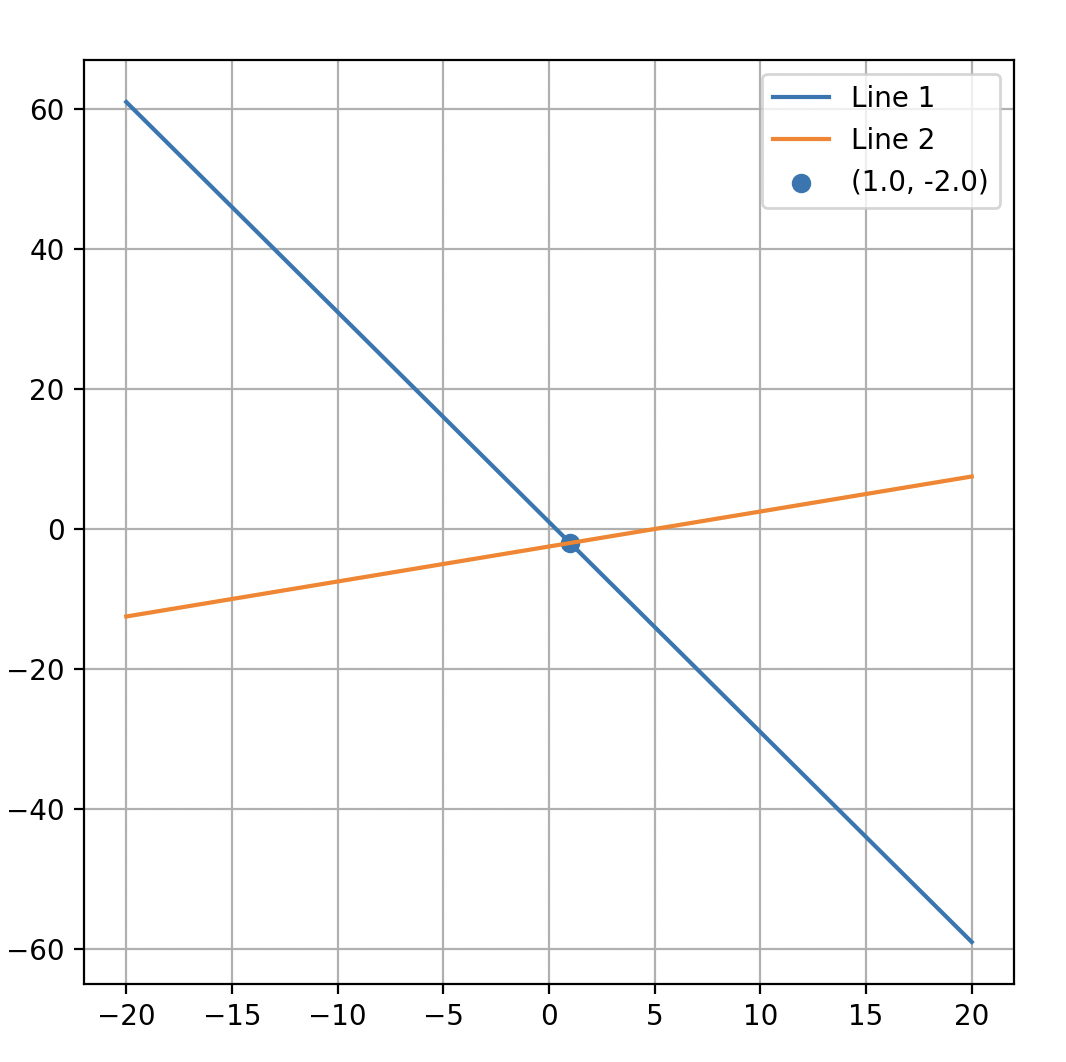
\includegraphics[width=0.6\columnwidth]{Figs/5338.png}
    \caption{Plot}
    \label{fig:placeholder}
\end{figure}
\end{document}
\end{frame}

\begin{frame}[fragile]
    \frametitle{Python Code}

    \begin{lstlisting}
import numpy as np
import numpy.linalg 
import matplotlib.pyplot as plt

answer = numpy.linalg.solve([[3,1],[-1,2]], [1,-5])

answer[0] = round(answer[0],2)
answer[1] = round(answer[1],2)
print(answer)
\end{lstlisting} 
\end{frame}

\begin{frame}[fragile]
    \frametitle{Python Code}

    \begin{lstlisting}


fig = plt.figure(figsize =(6,6))
ax = fig.add_subplot(111)

X = np.linspace(-20,20,2)

Y1 = (1-3*X)
Y2 = 0.5*(X-5)

ax.plot(X, Y1, label='Line 1')
ax.plot(X, Y2, label='Line 2')
ax.scatter(answer[0], answer[1], label=f'({answer[0]}, {answer[1]})')
ax.grid(True)
ax.legend()
plt.show()

    \end{lstlisting}
\end{frame}

\begin{frame}[fragile]
\frametitle{Plot}

\begin{figure}[H]
    \centering
    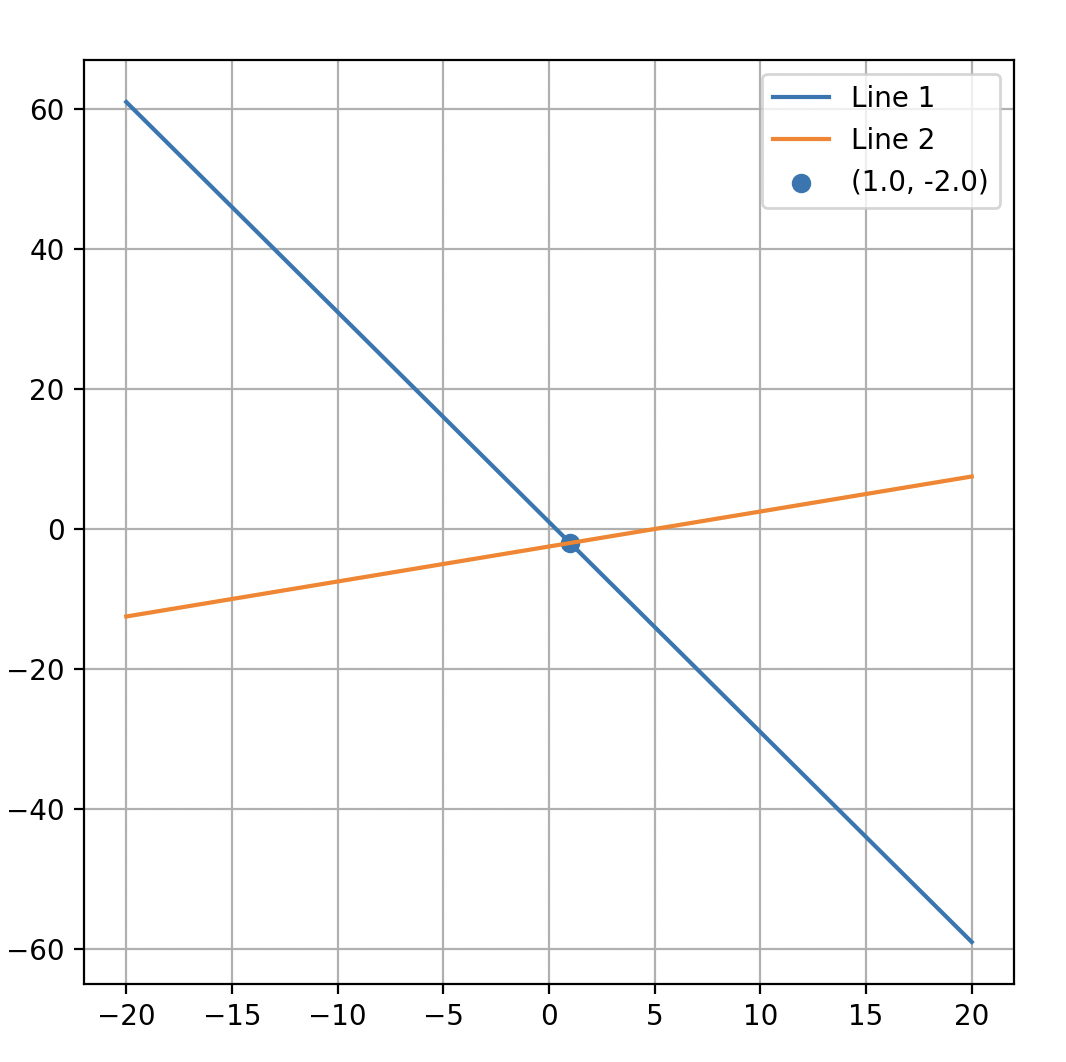
\includegraphics[width=0.6\columnwidth]{Figs/5338.png}
    \caption{Plot}
    \label{fig:placeholder}
\end{figure}

\end{frame}
\end{document}